\chapter{Results}

In this chapter we will show the results obtained in this work. They will be divided between the three metrics we chose to monitor (see section Experiment Design in the Development chapter).

\section{Rasterization Baseline}
First of all and as a sanity check, we will compare the performance of a renderer using ray tracing to one drawing the same geometry through rasterization. The model chosen for this will be the Viking Room from the Vulkan Tutorial \cite{VulkanTutorial}.

In the first place we will look at how video memory usage changes as the frame sizes get bigger. We can see a comparison of how much memory both renderers employ in graph \ref{memory-usage-comparison-graph}. We see an expected increase in memory consumption as the frame buffer resolutions get bigger, as well as a huge difference, of about an order of magnitude, between the two methods for any given resolution. This is to be expected not only because a bigger frame buffer will require more memory to be stored, but also because the ray tracer requires to store an acceleration structure as well as all the possible shaders bound at the same time.

\begin{figure}[hbt!]
    \centering
    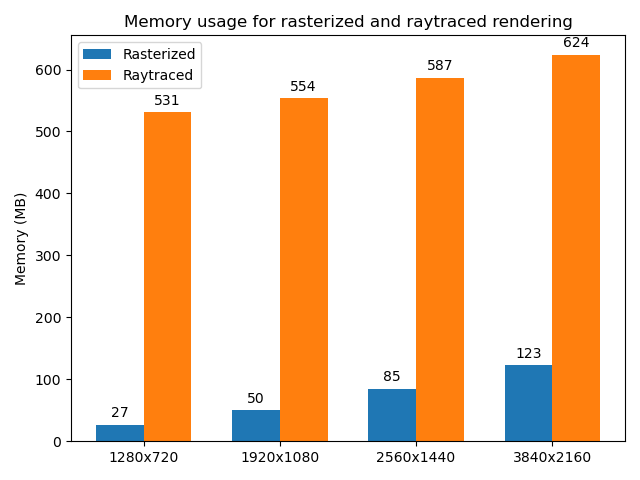
\includegraphics[width=1.0\textwidth]{figuras/vulkan-memory-usage-comparison.png}
    \caption{GPU memory consumption when rendering the Viking Room 3D model at a range of reasonable resolutions, using ray traced and traditionally rasterized graphics. We can see a significant difference between the two, as well as an expected increase as resolutions get higher.}
    \label{memory-usage-comparison-graph}
\end{figure}

Rasterized renderers have an initialization process quite different than raytraced ones since they do not make use of an acceleration structure. Therefore, we cannot compare it's building time in this context.

To finish this part, we will compare frame times from both renderers in the same fashion as the memory usage one: with the same model (Viking Room), we'll run them for 1000 frames and take the average time it took to render them at different screen resolutions. We can see how they stack up in figure \ref{frametimes-comparison-graph}. This is very similar to the memory usage comparison in that both frame times increase as the frame buffer resolution grows, with the rasterized renderer finishing the job much quicker than it's counterpart. In any case, in this instance the performance difference is even more exaggerated between the two, with rasterized graphics greatly surpassing ray traced ones.

\begin{figure}[hbt!]
    \centering
    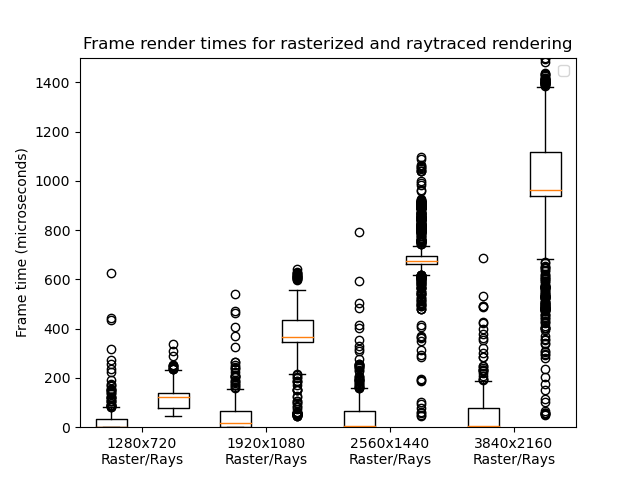
\includegraphics[width=1.0\textwidth]{figuras/vulkan-frametimes-comparison.png}
    \caption{Single frame rendering time when drawing the Viking Room 3D model at a range of reasonable resolution, using ray traced and traditionally rasterized graphics. As with the memory consumption graph, we see how the two of them take longer to finish in higher resolutions, while the rasterized renderer greatly outperforms the ray traced one.}
    \label{frametimes-comparison-graph}
\end{figure}

\section{Memory Usage}
To start the real comparison between Vulkan and OptiX we will look at the memory usage in GPU across both libraries, all models and all resolutions. We can see how much each model consumes in graph \ref{memory-usage-raytraced-comparison-graph}.

This is the first example of a trend we will start seeing throughout this chapter. Vulkan, either despite or thanks to it's explicitness when developing applications, is able to load and render the same ammount of geometry and detail as OptiX while requiring only a fraction of the resources, in this case video memory. This remains true while increasing the frame buffer size, with both libraries increasing the required memory at a similar rate. One last remarkable thing is how the results stack up to one another in the Hairball test case. Here we see how the memory consumed for both libraries is very similar, which suggests the two technologies tend to use a similar ammount of resources when triangle counts tend to infinity.

\begin{figure}
    \subfloat[BMW]{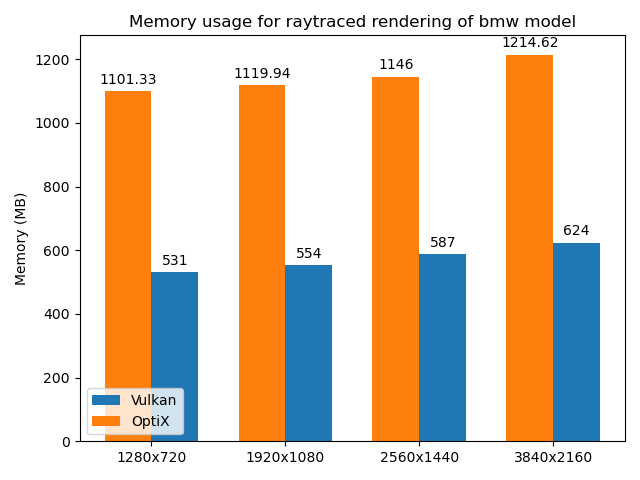
\includegraphics[width = 3in]{figuras/bmw-memory-usage-comparison.png}}
    \subfloat[Sponza]{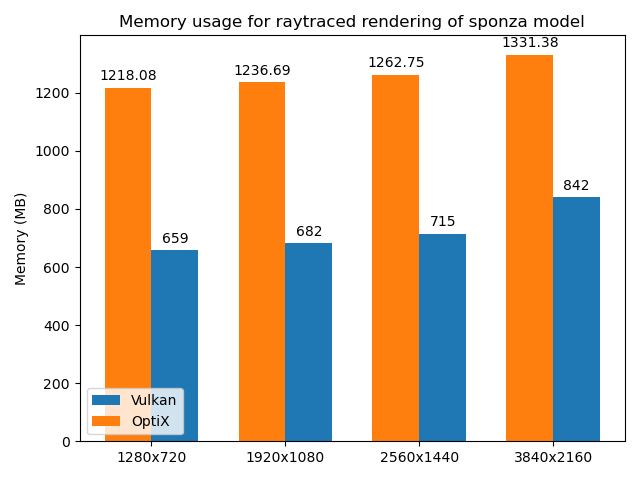
\includegraphics[width = 3in]{figuras/sponza-memory-usage-comparison.png}}\\
    \centering
    \subfloat[Hairball]{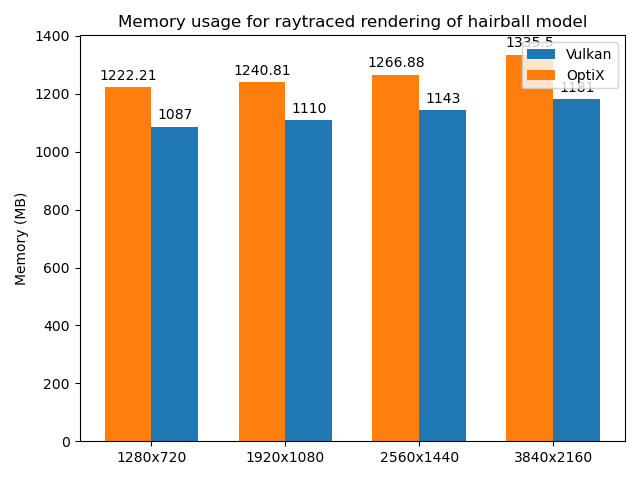
\includegraphics[width = 3in]{figuras/hairball-memory-usage-comparison.png}}
    \caption{Memory consumption of OptiX and Vulkan (raytraced) when rendering the 3D models BMW, Sponza and Hairball.}
    \label{memory-usage-raytraced-comparison-graph}
\end{figure}
\section{Acceleration Structure Build Time}
\section{Frame Time}
